\chapter{Shaft Design}
\section{Nomenclature}
\begin{tabular}[t]{lp{6.5cm}}
	$ [s] $ & permissible safety factor\\
	$ [\sigma] $ & permissible static strength, $ \unit{MPa} $\\
	$ [\tau] $ & permissible torsion, $ \unit{MPa} $\\
	$ a_w $ & shaft distance, $ \unit{mm} $\\
	$ b_O $ & rolling bearing width, $ \unit{mm}$\\
	$ \text{cb} $ & role of gear on the shaft (active or passive)\\
	$ \text{cq} $ & rotational direction of the shaft\\
	$ d $ & base shaft diameter, $ \unit{mm} $\\
	$ d_w $ & gear diameter, $ \unit{mm} $\\
	$ F_a $ & axial force, $ \unit{N} $\\
	$ F_r $ & radial force, $ \unit{N} $\\
	$ F_t $ & tangential force, $ \unit{N} $\\
	$ F_x $ & applied force, $ \unit{N} $\\	
\end{tabular}
\begin{tabular}[t]{lp{6.5cm}}
	$ h_n $ & distance between bearing lid and bolt, $ \unit{mm} $\\
	$ \text{hr} $ & tooth direction\\
	$ K_x $ & surface tension concentration factor\\
	$ K_y $ & diminish factor\\
	$ K_\sigma $ & combined influence factor in tension\\
	$ K_\tau $ & combined influence factor in shear\\
	$ \tilde{k}_1 $ & distance between elements, $ \unit{mm} $\\
	$ \tilde{k}_2 $ & distance between bearing surface and inner walls of the gearbox, $ \unit{mm} $\\
\end{tabular}\newpage
\begin{tabular}[t]{lp{6.5cm}}
	$ \tilde{k}_3 $ & distance between element surface and bearing lid, $ \unit{mm} $\\
	$ k_\sigma $ & fatigue stress concentration factor in tension\\
	$ k_\tau $ & fatigue stress concentration factor in shear\\
	$ l $ & length (general), $ \unit{mm} $\\
	$ l_m $ & hub length (general), $ \unit{mm} $\\
	$ M $ & moment at the cross section, $ \unit{N\cdot mm} $\\
	$ M_e $ & equivalent moment, $ \unit{N\cdot mm} $\\
	$ l_m $ & hub diameter, $ \unit{mm} $\\
	$ q $ & standardized coefficient of shaft diameter\\
	$ R $ & reaction force, $ \unit{N} $\\
	$ r $ & shoulder fillet radius, $ \unit{mm} $\\
	$ \bar{r} $ & position of applied force on the shaft, $\unit{mm}$\\
	$ S $ & length defined by table (6.1), $ \unit{mm} $\\
	$ s $ & calculated safety factor\\
	$ s_\sigma $ & safety factor in tensile stress\\
	$ s_\tau $ & safety factor in shear stress\\
	$ T $ & torque at the cross section, $ \unit{N\cdot mm} $\\
\end{tabular}
\begin{tabular}[t]{lp{6.5cm}}
	$ W $ & section modulus, $ \unit{mm^3} $\\
	$ W_O $ & polar section modulus, $ \unit{mm^3} $\\
	$ \alpha_{tw} $ & traverse meshing angle, $ ^\circ $\\
	$ \beta $ & helix angle, $ ^\circ $\\
	$ \psi_\sigma $ & mean stress influence factor\\
	$ \psi_\tau $ & mean shear influence factor\\
	$ \sigma_{-1} $ & endurance limit at stress ratio of -1, $ \unit{MPa} $\\
	$ \sigma_a $ & tensile stress amplitude, $ \unit{MPa} $\\
	$ \sigma_b $ & ultimate strength, $ \unit{MPa} $\\
	$ \sigma_{ch} $ & yield limit, $ \unit{MPa} $\\
	$ \sigma_m $ & mean tensile stress, $ \unit{MPa} $\\
	$ \sigma_{td} $ & static strength, $ \unit{MPa} $\\
	$ \tau_{-1} $ & endurance limit at shear ratio of -1, $ \unit{MPa} $\\
	$ \tau_a $ & shear stress amplitude, $ \unit{MPa} $\\
	$ \tau_m $ & mean shear stress, $ \unit{MPa} $\\
	$ _1 $ & subscript for shaft 1\\
	$ _2 $ & subscript for shaft 2\\
	$ _{max} $ & subscript for maximum value\\
	$ _{sh1} $ & subscript for shaft 1\\
	$ _{sh2} $ & subscript for shaft 2\\
	$ _x $ & subscript for x-axis\\
	$ _y $ & subscript for y-axis\\
	$ _z $ & subscript for z-axis\\
\end{tabular}

\section{Choose material}
For moderate load, we will use quenched 45X steel to design the shafts. From table (6.1), the specifications are as follows: $ S \leq 100\unit{(mm)} $, HB260, $ \sigma_b = 850\unit{(MPa)}$, $ \sigma_{ch} = 650\unit{(MPa)}$. 

\section{Transmission Design}
\subsection{Load on shafts}
\subsubsection{Applied forces from Gears}
Following p.186, the subscript convention of the book will be used in this chapter. If a symbol has 2 numeric subscripts, the first one is the ordinal number of shafts while the second one is used for machine elements.\\
On shaft 1, the motor is labeled 1 and the pinion is labeled 2. On shaft 2, the driven gear is labeled 1 and the driving sprocket is labeled 2. Therefore, we obtain:\\
$ \bar{r}_{12} = -d_{w12}/2 \approx -20.83\unit{(mm)}$, $ \text{hr}_{12} = +1 $, $ \text{cb}_{12} = +1 $, $ \text{cq}_1 = +1 $\\
$ \bar{r}_{21} = +d_{w21}/2 \approx +104.17\unit{(mm)}$, $ \text{hr}_{21} = -1 $, $ \text{cb}_{21} = -1$, $ \text{cq}_2 = -1$
\paragraph{Find magnitude of $ F_{t} $, $ F_r $, $ F_a $}
Using the results from the previous chapter: , $ \beta_w = 13.59^\circ $, $ d_{w12}\approx 41.67\unit{(mm)} $
\[
\left\{ 
\begin{array}{l@{{}={}}l@{{}={}}l}
F_{t12}& F_{t21}& \dfrac{2T_{sh1}}{d_{w12}}\approx 2402.28\unit{(N)}\\
F_{r12}& F_{r21}&  \dfrac{F_{t12}\tan\alpha}{\cos\beta_w}\approx 925.46 \unit{(N)}\\
F_{a12}& F_{a21}& F_{t12}\tan\beta_w\approx 580.75 \unit{(N)}\\ 
\end{array}
\right.
\]
\paragraph{Find direction of $ F_{t} $, $ F_r $, $ F_a $}
Following the sign convention, we obtain the forces:
\[
\left\{ 
\begin{array}{l@{{}={}}l}
F_{x12}& \dfrac{\bar{r}_{12}}{|\bar{r}_{12}|}\text{cq}_1\text{cb}_{12}F_{t12}\approx -2402.28 \unit{(N)}\\
F_{y12}& -\dfrac{\bar{r}_{12}}{|\bar{r}_{12}|}\dfrac{\tan\alpha}{\cos\beta_w}F_{t12}\approx 925.46 \unit{(N)}\\
F_{z12}& \text{cq}_1\text{cb}_{12}\text{hr}_{12}F_{t12}\tan\beta_w\approx 580.75 \unit{(N)}\\ 
\end{array}
\right.
\]
\[
\left\{ 
\begin{array}{l@{{}={}}l}
F_{x21}& \dfrac{\bar{r}_{21}}{|\bar{r}_{21}|}\text{cq}_2\text{cb}_{21}F_{t21}\approx 2402.28 \unit{(N)}\\
F_{y21}& -\dfrac{\bar{r}_{21}}{|\bar{r}_{21}|}\dfrac{\tan\alpha_{tw}}{\cos\beta_w}F_{t21}\approx -925.46 \unit{(N)}\\
F_{z21}& \text{cq}_2\text{cb}_{21}\text{hr}_{21}F_{t21}\tan\beta_w\approx -580.75 \unit{(N)}\\ 
\end{array}
\right.
\]

\subsubsection{Applied forces from Chain drives}
Assuming the angle between x-axis and $ F_r $ is $ 210^\circ $ and $ F_r \approx 2678.96 \unit{(N)} $ (chapter 2), we get the direction of $ F_r $ on shaft 2:
\[
\left\{ 
\begin{array}{l@{{}={}}l}
F_{x22}& F_{r22}\cos210^\circ\approx -2320.05 \unit{(N)}\\
F_{y22}& F_{r22}\sin210^\circ\approx -1339.48 \unit{(N)}\\
\end{array}
\right.
\]

\subsection{Preliminary calculations}
Since shaft 1 and shaft 2 receive input torques $ T_{sh1} $ and $ T_{sh2} $, respectively, $ [\tau_1] = 15\unit{(MPa)}$ and $ [\tau_2]=30\unit{(MPa)} $. Using equation (10.9), we can approximate the base shaft diameters $ d_1 $ and $ d_2 $:\vskip2mm
$ d_1 \geq \sqrt[3]{\dfrac{T_{sh1}}{0.2[\tau_1]}} \approx 25.55 \unit{(mm)}$\\
$ d_2 \geq \sqrt[3]{\dfrac{T_{sh2}}{0.2[\tau_2]}} \approx 34.1 \unit{(mm)}$\vskip2mm
Recall that our motor is 4A160M2Y3, inspecting table P1.7 we obtain the motor's output shaft diameter is $ 42 \unit{(mm)} $. According to the recommendations on p.189, we limit the chosen range of $ d_1 \geq (0.8\div1.2)\times 42\unit{(mm)} $. For $ d_2 $, the chosen range must be around $ (0.3\div0.35)\times a_w\unit{(mm)}$. Thus, $ d_1 = 35\unit{(mm)} $, $ d_2 = 40\unit{(mm)} $. Consulting table (10.2) gives $ b_{O1} \approx 21\unit{(mm)} $ and $ b_{O2} \approx 23\unit{(mm)} $

\subsection{Identify the distance between bearings and applied forces}

\begin{figure}[ht]
	\centering	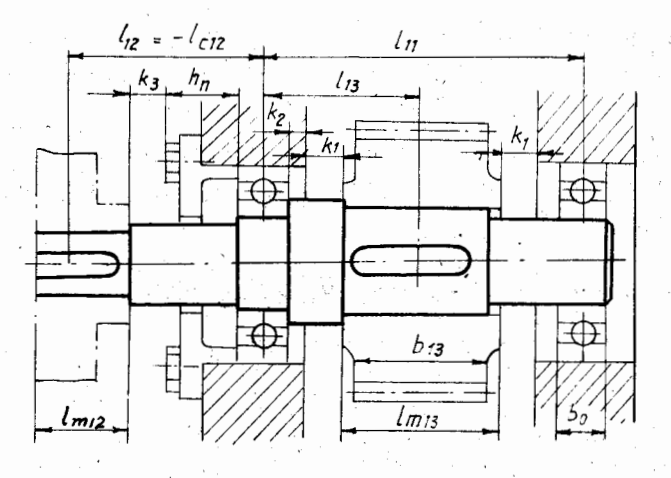
\includegraphics[width=150mm]{shaft1.png}
	\caption{Shaft design and its dimensions}
	\label{shaft}
\end{figure}

In this section, we will find all the parameters in Figure \ref{shaft}. However, if a parameter has 2 numeric subscripts, the first one will denote the ordinal number of shafts.\\
Using equation (10.10), the gear hubs are $ l_{m13} = l_{m12} = 1.5d_1 =  45\unit{(mm)} $, $ l_{m23} = l_{m22} = 1.5d_2 = 52.5\unit{(mm)} $, where $ l_{m22} $ is the chain hub.\\
From table (10.3), we choose $ \tilde{k}_1=10\unit{(mm)}$, $ \tilde{k}_2=8\unit{(mm)} $, $ \tilde{k}_3=15\unit{(mm)} $, $ h_n=18\unit{(mm)} $. This parameters apply for both shafts in the system.\\
Table (10.4) introduces the formulas for several types of gearbox. Since our system only concerns about 1-level gear reducer, the ones below are used:\\
On shaft 1:\\
$ l_{12} = -l_{c12} = -\left[ 0.5(l_{m12}+b_{O1})+\tilde{k}_3+h_n  \right] = -71.5 \unit{(mm)} $\\
$ l_{13} = 0.5(l_{m13}+b_{O1})+\tilde{k}_1+\tilde{k}_2 = 59.5 \unit{(mm)} $\\
$ l_{11} = 2l_{13} = 119 \unit{(mm)}$\\
On shaft 2:\\
$ l_{22} = -l_{c22} = -\left[ 0.5(l_{m22}+b_{O2})+\tilde{k}_3+h_n \right] = -66.75 \unit{(mm)} $\\
$ l_{23} = 0.5(l_{m23}+b_{O2})+\tilde{k}_1+\tilde{k}_2 = 54.75 \unit{(mm)} $\\
$ l_{21} = 2l_{23} = 109.5 \unit{(mm)}$

% this part is incorrect
\subsection{Determine shaft diameters and lengths}

\paragraph{Find reaction forces}

\begin{figure}[ht]
	\centering
	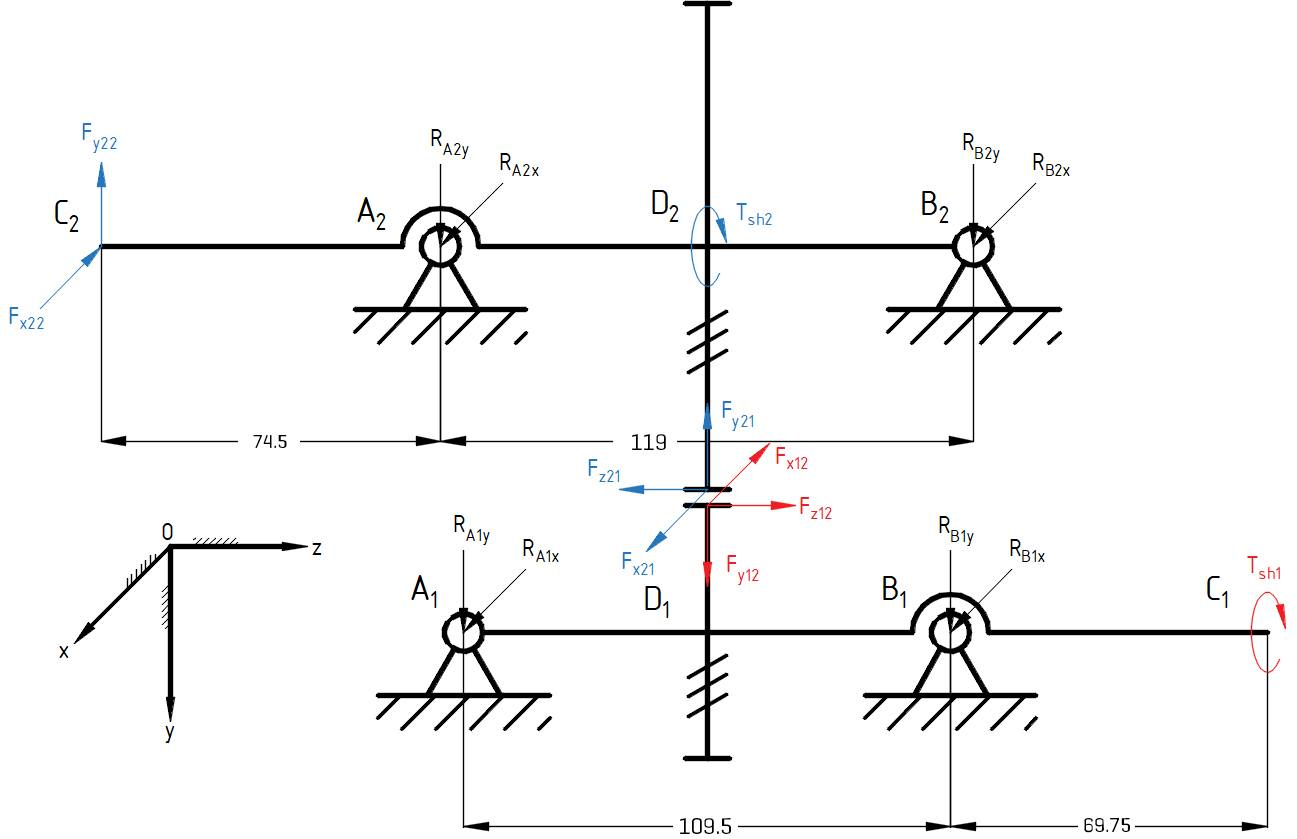
\includegraphics[width=160mm]{shaft.png}
	\caption{Force analysis of 2 shafts}
	\label{force on shaft}
\end{figure}

From the diagram, we solve for the reaction forces at $ A_1 $, $ A_2 $, $ B_1 $, $ B_2 $, which are $ R_{A1x} $, $ R_{A1y} $, $ R_{B1x} $, $ R_{B1y} $, $ R_{A2x} $, $ R_{A2y} $, $ R_{B2x} $, $ R_{B2y} $. Using equilibrium conditions
\[
\left\{ 
\begin{array}{l@{{}={}}l}
\displaystyle\sum_{i} \mathbf{F_{i}} & 0\\
\displaystyle\sum_{i} \mathbf{r_i}\times \mathbf{F_i}& 0\\
\end{array}
\right.
\]
we obtain the results:\vskip2mm
%\begin{table}[ht]
{\centering
	\begin{tabular}[ht]{p{7cm}p{7cm}}
		$
		\left\{ 
		\begin{array}{l@{{} \approx {}}l}
		R_{A1x} & 1201.14\unit{(N)}\\
		R_{A1y} & -352.24\unit{(N)}\\
		R_{B1x} & 1201.14\unit{(N)}\\
		R_{B1y} & -573.22\unit{(N)}\\
		\end{array}
		\right.
		$ & $
		\left\{ 
		\begin{array}{l@{{} \approx {}}l}
		R_{A2x} & 943.15\unit{(N)}\\
		R_{A2y} & 3668.4 \unit{(N)}\\
		R_{B2x} & -2005.96 \unit{(N)}\\
		R_{B2y} & -422.89 \unit{(N)}\\
		\end{array}
		\right.
		$
\end{tabular}}\vskip2mm
The total bending moments at 8 critical cross sections are also calculated (we use the formula (10.15) to derive $M=\sqrt{M_x^2+M_y^2}$ at each section):\vskip2mm
{\centering
	\begin{tabular}[ht]{p{7cm}p{7cm}}
		$
		\left\{ 
		\begin{array}{l@{{} \approx {}}l}
		M_{A1} & 0 \unit{(N\cdot mm)}\\
		M_{D1}^- & 68531.85 \unit{(N\cdot mm)}\\
		M_{D1}^+ & 72867.4 \unit{(N\cdot mm)}\\
		M_{B1} & 0 \unit{(N\cdot mm)}\\
		M_{C1} & 0 \unit{(N\cdot mm)}\\
		\end{array}
		\right.
		$ &
		$
		\left\{ 
		\begin{array}{l@{{} \approx {}}l}
		M_{C2} & 0 \unit{(N\cdot mm)}\\
		M_{A2} & 191545.76 \unit{(N\cdot mm)}\\
		M_{D2}^- & 146910 \unit{(N\cdot mm)}\\
		M_{D2}^+ & 121977.78 \unit{(N\cdot mm)}\\
		M_{B2} & 0 \unit{(N\cdot mm)}\\
		\end{array}
		\right.
		$
\end{tabular}}\vskip2mm

\paragraph{Draw bending moment - torque diagrams} Knowing the reaction forces, we can easily draw bending moment and torque diagram for both shafts on 2 major planes (xOz) and (yOz).

\begin{figure}[ht]
	\centering
	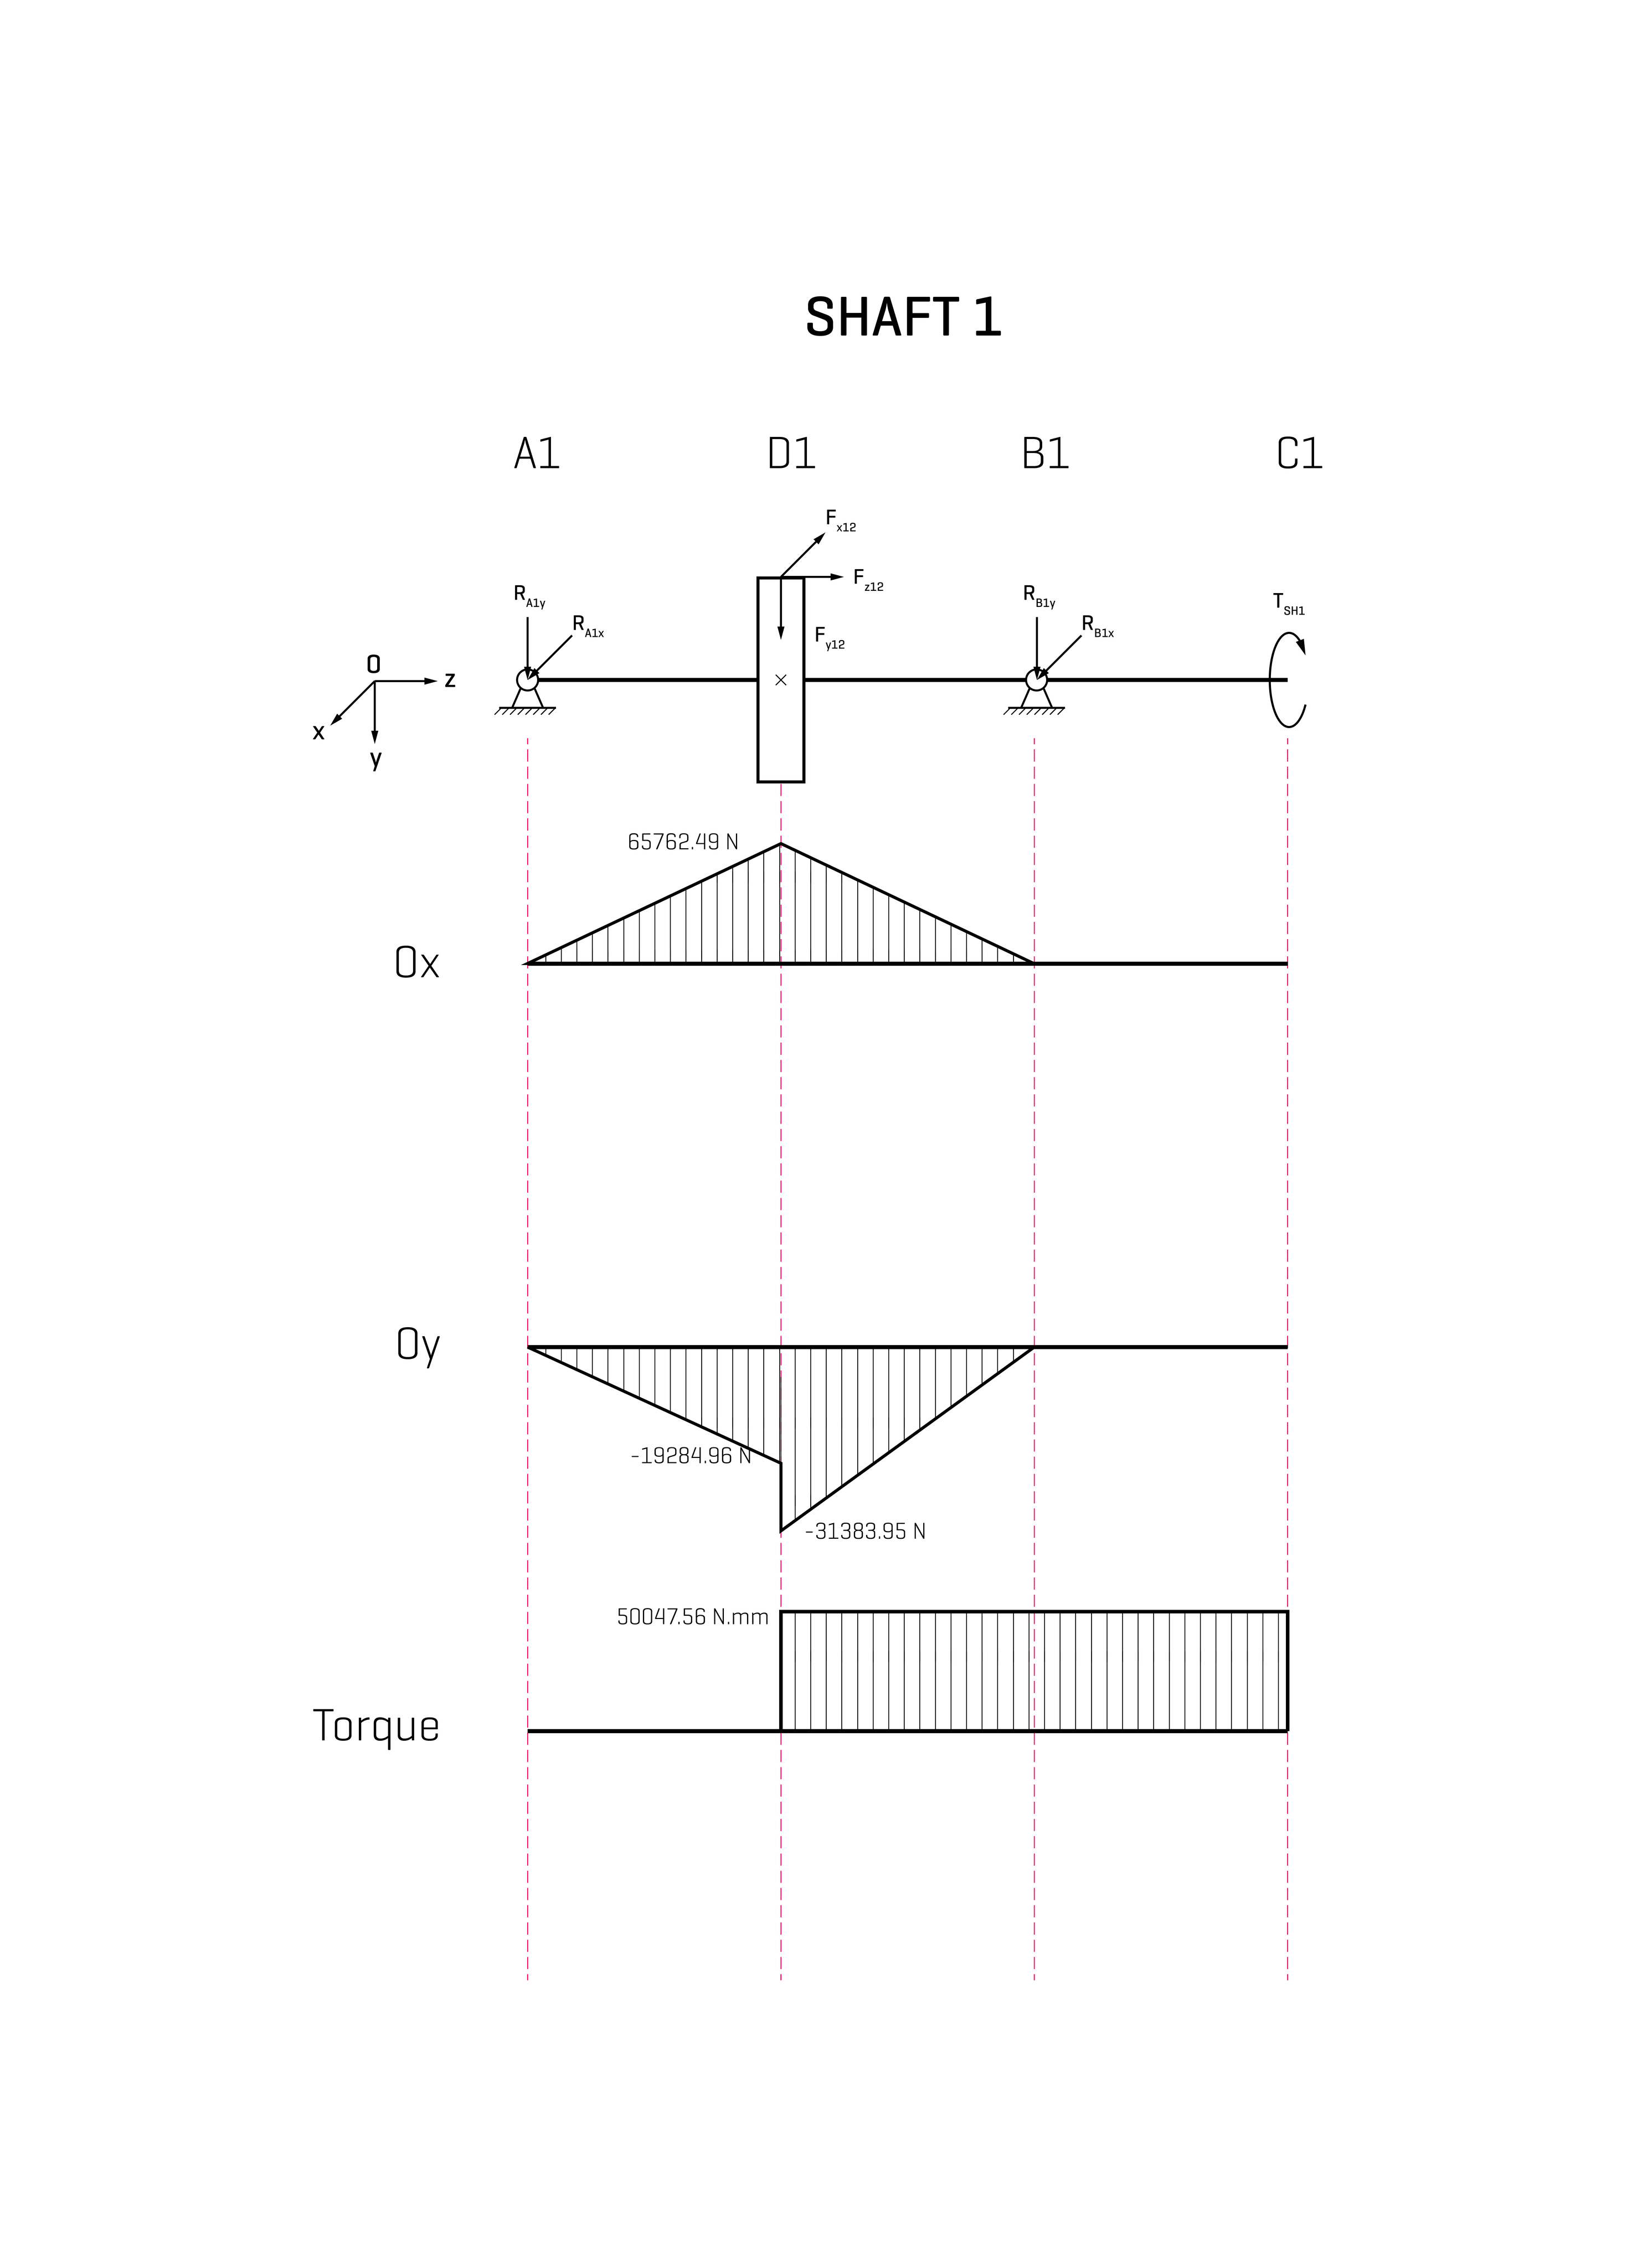
\includegraphics[width=160mm]{mshaft1.png}
	\caption{Bending moment-torque diagram of shaft 1}
	\label{mshaft1}
\end{figure}

\begin{figure}[ht]
	\centering
	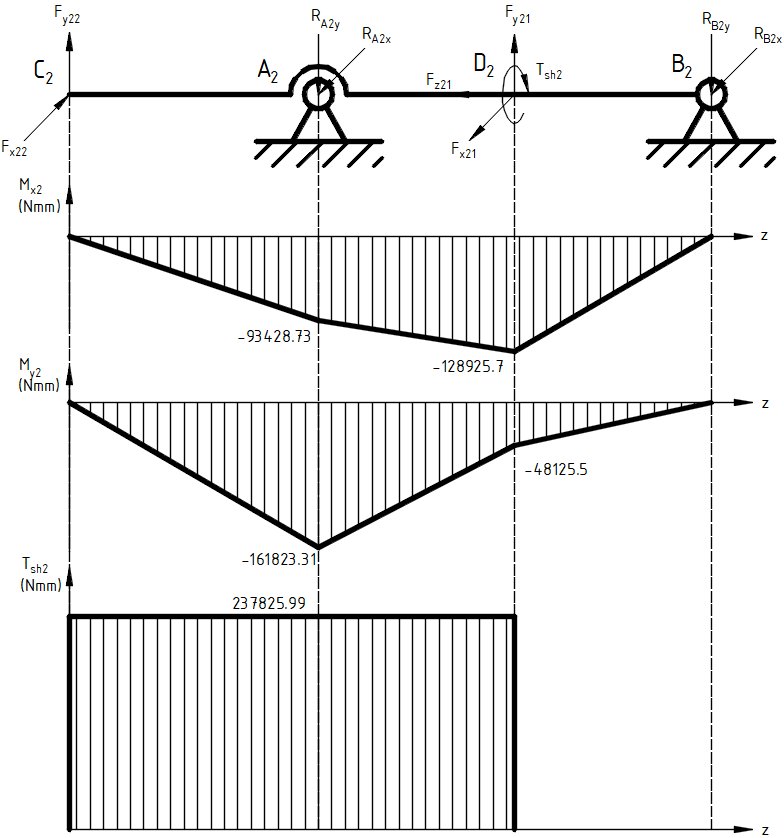
\includegraphics[width=153mm]{mshaft2.png}
	\caption{Bending moment-torque diagram of shaft 2}
	\label{mshaft2}
\end{figure}

\paragraph{Find equivalent moments} Knowing $ T_{sh1} $ and $ T_{sh2} $, we calculate equivalent moment $ M_e $ at the 8 cross sections specified using the formula below:
\[M_e = \sqrt{M_x^2 + M_y^2 + 0.75T_{sh}^2}\]

%\begin{table}[ht]
%	\centering
\begin{tabular}{p{7cm}p{7cm}}
	$
	\left\{ 
	\begin{array}{l@{{} \approx {}}l}
	M_{eA1} & 0 \unit{(N\cdot mm)}\\
	M_{eD1}^- & 81087.5 \unit{(N\cdot mm)}\\
	M_{eD1}^+ & 84783.4 \unit{(N\cdot mm)}\\
	M_{eB1} & 43342.46 \unit{(N\cdot mm)}\\
	M_{eC1} & 43342.46 \unit{(N\cdot mm)}\\
	\end{array}
	\right.
	$ &
	$
	\left\{ 
	\begin{array}{l@{{} \approx {}}l}
	M_{eC2} & 205963.35 \unit{(N\cdot mm)}\\
	M_{eA2} & 281266.2 \unit{(N\cdot mm)}\\
	M_{eD2}^- & 252989.03 \unit{(N\cdot mm)}\\
	M_{eD2}^+ & 239373.1 \unit{(N\cdot mm)}\\
	M_{eB2} & 0 \unit{(N\cdot mm)}\\
	\end{array}
	\right.
	$
\end{tabular}\vskip2mm
%\end{table}

\paragraph{Find permissible stress}
$ [\sigma_1] $ and $ [\sigma_2] $ are determined by table (10.5). Since we use quenched 45X steel, $ [\sigma_1] = 67 \unit{(MPa)}$ and $ [\sigma_2] = 64 \unit{(MPa)}$ ($ [\sigma_2] $ is achieved using interpolation).

\paragraph{Find standardized diameters at specific locations on the shaft} Having $ M_e $ and $ [\sigma] $, the next step is to estimate specific diameter at the key points mentioned above using equation (10.17) on p.194, which only applies for rigid shafts:
\[d \geq \sqrt[3]{\dfrac{M_e}{0.1[\sigma]}}\]

\begin{tabular}{p{7cm}p{7cm}}
	$
	\left\{ 
	\begin{array}{l@{{} \approx {}}l}
	d_{A1} & 0 \unit{(mm)}\\
	d_{D1} & 23.66 \unit{(mm)}\\
	d_{B1} & 18.92 \unit{(mm)}\\
	d_{C1} & 18.92 \unit{(mm)}\\
	\end{array}
	\right.
	$ &
	$
	\left\{ 
	\begin{array}{l@{{} \approx {}}l}
	d_{C2} & 32.32 \unit{(mm)}\\
	d_{A2} & 35.86 \unit{(mm)}\\
	d_{D2} & 34.61 \unit{(mm)}\\
	d_{B2} & 0\unit{(mm)}\\
	\end{array}
	\right.
	$
\end{tabular}

T\text{hr}ough rough calculations, we will choose the diameters according to standards given on p.195 (one applies for bearings while the other is used for the remaining machine elements):

\begin{tabular}{p{7cm}p{7cm}}
	$
	\left\{ 
	\begin{array}{l@{{} = {}}l}
	d_{A1} & 35 \unit{(mm)}\\
	d_{D1} & 24 \unit{(mm)}\\
	d_{B1} & 35 \unit{(mm)}\\
	d_{C1} & 19 \unit{(mm)}\\
	\end{array}
	\right.
	$ &
	$
	\left\{ 
	\begin{array}{l@{{} = {}}l}
	d_{C2} & 34 \unit{(mm)}\\
	d_{A2} & 40 \unit{(mm)}\\
	d_{D2} & 36 \unit{(mm)}\\
	d_{B2} & 40 \unit{(mm)}\\
	\end{array}
	\right.
	$
\end{tabular}

\section{Fatigue Strength Analysis}
For each critical point, the fatigue strength there must satisfy this condition:
\[s=\dfrac{s_\sigma s_\tau}{\sqrt{s_\sigma^2+s_\tau^2}}\geq[s]\]
\begin{tabular}{ll}
	where & $ s_\sigma = \dfrac{\sigma_{-1}}{K_\sigma\sigma_a + \psi_\sigma\sigma_m}$\\
	& $ s_\tau = \dfrac{\tau_{-1}}{K_\tau\tau_a + \psi_\tau\tau_m}$
\end{tabular}\\\\
Assuming the surfaces are smooth, properly ground and quenched by high frequency voltage, we obtain $ K_x = 1 $ from table (10.8) and $ K_y = 1.4 $ from table (10.9), where $ [\sigma_b] = 850 \unit{(MPa)} $ is the property of quenched 45X steel.

\paragraph{Find $ \sigma_{-1}$, $ \tau_{-1} $} Using formulas on p.196:\\
$ \sigma_{-1} = 0.35[\sigma_b] + 120 \approx 417.5 \unit{(MPa)} $\\
$ \tau_{-1} \approx 0.58\sigma_{-1} \approx 242.15 \unit{(MPa)} $

\paragraph{Find $ \sigma_{a}, \tau_{a}, \sigma_{m}, \tau_{m} $} For this part, we divide into 3 key points:
\begin{enumerate}
	\item For rotating shaft, $ \sigma_{m} = 0, \sigma_a = \dfrac{\sqrt{M_x^2+M_y^2}}{W} $ (equation (10.22)), where $ M_x $ and $ M_y $ are at the cross section of interest.
	\item By design, the shafts only rotate in one direction, thus $ \tau_m = \tau_a = \dfrac{T_{sh}}{2W_O} $ (equation (10.23)).
	\item We also assume the shafts have circular cross section, which makes $ W = \dfrac{\pi d^3}{32} $ and $ W_O = \dfrac{\pi d^3}{16} $ according to table (10.6), where $ d $ is the diameter of a cross section of the shaft.
\end{enumerate}
The table below shows the results after calculation:
\begin{table}[ht]
	\centering
	\begin{tabular}{|
			>{\columncolor[HTML]{C0C0C0}}l |l|l|l|l|l|l|l|}
		\hline
		&
		\cellcolor[HTML]{C0C0C0}\begin{tabular}[c]{@{}l@{}}$d$\\ $\unit{(mm)}$\end{tabular} &
		\cellcolor[HTML]{C0C0C0}\begin{tabular}[c]{@{}l@{}}$W$\\ $\unit{(mm^3)}$\end{tabular} &
		\cellcolor[HTML]{C0C0C0}\begin{tabular}[c]{@{}l@{}}$W_O$\\ $\unit{(mm^3)}$\end{tabular} &
		\cellcolor[HTML]{C0C0C0}\begin{tabular}[c]{@{}l@{}}$\sigma_m$\\ $\unit{(MPa)}$\end{tabular} &
		\cellcolor[HTML]{C0C0C0}\begin{tabular}[c]{@{}l@{}}$\sigma_{a}$\\ $\unit{(MPa)}$\end{tabular} &
		\cellcolor[HTML]{C0C0C0}\begin{tabular}[c]{@{}l@{}}$\tau_m$\\ $\unit{(MPa)}$\end{tabular} &
		\cellcolor[HTML]{C0C0C0}\begin{tabular}[c]{@{}l@{}}$\tau_{a}$\\ $\unit{(MPa)}$\end{tabular} \\ \hline
		$A_1$ & 20 & 785.4   & 1570.8   & 0 & 0     & 15.93 & 15.93 \\ \hline
		$D_1$ & 24 & 1357.17 & 2714.34  & 0 & 49.2  & 9.22  & 9.22  \\ \hline
		$B_1$ & 20 & 785.4   & 1570.8   & 0 & 0     & 15.93 & 15.93 \\ \hline
		$C_1$ & 19 & 673.38  & 1346.76  & 0 & 0     & 18.58 & 18.58 \\ \hline
		$C_2$ & 32 & 3216.99 & 6433.98  & 0 & 0     & 18.48 & 18.48 \\ \hline
		$A_2$ & 40 & 6283.19 & 12566.37 & 0 & 29.74 & 9.46  & 9.46  \\ \hline
		$D_2$ & 34 & 3858.66 & 7717.32  & 0 & 36.67 & 15.41 & 15.41 \\ \hline
		$B_2$ & 35 & 4209.24 & 8418.49  & 0 & 0     & 14.13 & 14.13 \\ \hline
	\end{tabular}
	\caption{Calculated variables for $ \sigma_{a}, \tau_{a}, \sigma_{m}, \tau_{m} $}
\end{table} Since $ \sigma_b = 850 \unit{(MPa)}$ for both shafts, $ \psi_\sigma = 0.1 $ and $\psi_\tau = 0.05 $

\paragraph{Find $ K_{\sigma}, K_\tau $} We calculate $ K_{\sigma} $ using formula:
\[ K_{\sigma} = \left( \dfrac{k_\sigma}{\varepsilon_\sigma} + K_x - 1\right) K_y^{-1} \]
and $ K_\tau $ with:
\[ K_{\tau} = \left( \dfrac{k_\tau}{\varepsilon_\tau} + K_x - 1\right) K_y^{-1} \]
Table (10.10), (10.11) and (10.13) are examined to find $ \dfrac{k_\sigma}{\varepsilon_\sigma} $ ratio. Given $ [\sigma_H] = 850 \unit{(MPa)} $ base shaft diameters $ d_1 $ and $ d_2 $ are compared to the diameters at critical locations $ A $, $ B $, $ C $, $ D $. If the base shaft is smaller, table (10.10) and (10.11) are used. If it is larger, we will use table (10.13) instead; the concentration stress factor in this case is demonstrated in the figure:\\

%\begin{figure}[ht]
%	\centering
%	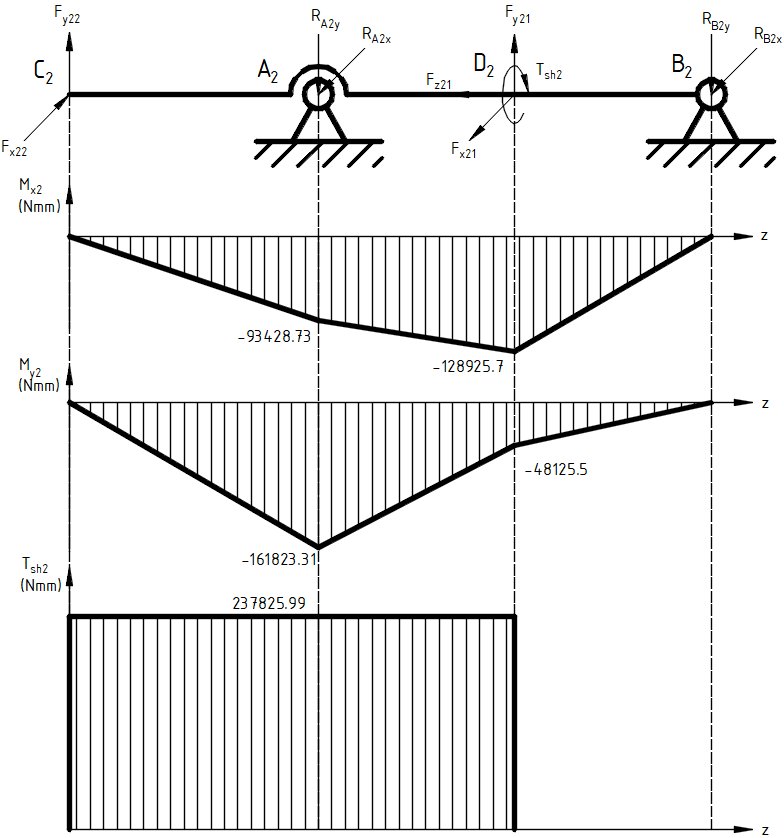
\includegraphics[width=153mm]{mshaft2.png}
%	\caption{Dimensions of the shaft at an critical area}
%	\label{concentration stress factor}
%\end{figure}

Final calculation is provided in the table:

\begin{table}[ht]
	\begin{tabular}{|l|l|l|l|l|l|l|l|l|l|l|l|l|}
		\hline
		\rowcolor[HTML]{C0C0C0} 
		&
		$d\unit{(mm)}$ &
		$r$ &
		$k_\sigma$ &
		$k_\tau$ &
		$\varepsilon_\sigma$ &
		$\varepsilon_\tau$ &
		$\frac{k_\sigma}{\varepsilon_\sigma}$ &
		$\frac{k_\tau}{\varepsilon_\tau}$ &
		$K_x$ &
		$K_y$ &
		$K_\sigma$ &
		$K_\tau$ \\ \hline
		\cellcolor[HTML]{C0C0C0}$A_1$ & 20 & 0.4  & 3 & 1.95 & 0.83 & 0.89 & 3.61 & 2.19 & 1 & 1.4 & 2.58 & 1.57 \\ \hline
		\cellcolor[HTML]{C0C0C0}$D_1$ & 24 & 0.48 & 3 & 1.95 & 0.81 & 0.85 & 3.7  & 2.29 & 1 & 1.4 & 2.65 & 1.64 \\ \hline
		\cellcolor[HTML]{C0C0C0}$B_1$ & 20 & 0.4  & 3 & 1.95 & 0.83 & 0.89 & 3.61 & 2.19 & 1 & 1.4 & 2.58 & 1.57 \\ \hline
		\cellcolor[HTML]{C0C0C0}$C_1$ & 19 & 0.38 & 3 & 1.95 & 0.84 & 0.89 & 3.57 & 2.19 & 1 & 1.4 & 2.55 & 1.57 \\ \hline
		\cellcolor[HTML]{C0C0C0}$C_2$ & 32 & 0.64 & 3 & 1.95 & 0.76 & 0.80 & 3.95 & 2.44 & 1 & 1.4 & 2.82 & 1.74 \\ \hline
		\cellcolor[HTML]{C0C0C0}$A_2$ & 40 & -    & - & -    & -    & -    & 3.34 & 2.46 & 1 & 1.4 & 2.39 & 1.76 \\ \hline
		\cellcolor[HTML]{C0C0C0}$D_2$ & 34 & 0.68 & 3 & 1.95 & 0.74 & 0.80 & 4 & 2.44 & 1 & 1.4 & 2.86 & 1.75 \\ \hline
		\cellcolor[HTML]{C0C0C0}$B_2$ & 35 & -    & - & -    & -    & -    & 3.3  & 2.44 & 1 & 1.4 & 2.36 & 1.74 \\ \hline
	\end{tabular}
	\caption{Calculated variables in $ K_\sigma $ and $ K_\tau $}
\end{table}
\paragraph{Find $ s_\sigma $, $ s_\tau $ and $ s $} Combining the results altogether, we obtain the following table:
\begin{table}[ht]
	\centering
	\begin{tabular}{|
			>{\columncolor[HTML]{C0C0C0}}l |p{2cm}|p{2cm}|p{2cm}|}
		\hline
		& \cellcolor[HTML]{C0C0C0}$s_\sigma$ & \cellcolor[HTML]{C0C0C0}$s_\tau$ & \cellcolor[HTML]{C0C0C0}$s$ \\ \hline
		$A_1$ & $\gg s_\tau$ & 9.41  & 9.41 \\ \hline
		$D_1$ & 3.21         & 16    & 3.14 \\ \hline
		$B_1$ & $\gg s_\tau$ & 9.41  & 9.41 \\ \hline
		$C_1$ & $\gg s_\tau$ & 8.07  & 8.07 \\ \hline
		$C_2$ & $\gg s_\tau$ & 7.32  & 7.32 \\ \hline
		$A_2$ & 5.88         & 14    & 5.43 \\ \hline
		$D_2$ & 3.99         & 8.77  & 3.63  \\ \hline
		$B_2$ & $\gg s_\tau$ & 9.56  & 9.56 \\ \hline
	\end{tabular}
	\caption{Safety factor at critical cross sections}
\end{table}\\
Since the smallest safety factor is at the cross section $ D_1 $, which has the value of $ 3.14 > [s] = 1.5 \div 2.5$, we can neglect rigidity analysis according to the conclusion on p.195.

\section{Static Strength Analysis}
Along with fatigue strength, static strength is also considered and every shaft must satisfy the following condition at critical cross sections (equation (10.27)):
\[\sigma_{e} = \sqrt{\left( \dfrac{M_{max}}{0.1d^3}\right)^2 + 3\left( \dfrac{T_{max}}{0.2d^3}\right) ^2} \leq [\sigma]\]
where $ M_{max}, T_{max} $ are the largest bending moment and torque at the cross section, respectively. Let $ [\sigma] \approx 0.8\sigma_{ch} = 520 \unit{(MPa)}$, the results are in the table below:
\begin{table}[ht]
	\centering
	\begin{tabular}{|l|l|l|l|l|l|l|l|l|}
		\hline
		\rowcolor[HTML]{C0C0C0} 
		& $A_1$ & $D_1$ & $B_1$ & $C_1$ & $C_2$ & $A_2$ & $D_2$ & $B_2$ \\ \hline
		\cellcolor[HTML]{C0C0C0}$\sigma_{e}\unit{(MPa)}$ & 54.18 & 57.59 & 54.18 & 63.19 & 62.86 & 43.45 & 63.58 & 48.04 \\ \hline
	\end{tabular}
	\caption{Calculated static strength at critical cross sections}
\end{table}\\
which satisfy the given condition.



%\paragraph{Find $ a_w $} On p.149, the following formula is used:
%\begin{equation}
%	a_w = (z_2+q)\sqrt[3]{\left( \dfrac{170}{z_2[\tau_H]}\right) ^2 \dfrac{T_2K_H}{q}}
%\end{equation}